\documentclass[11pt]{scrartcl}
\usepackage[utf8]{inputenc}
\usepackage{evank}


%% insert title here
\newcommand{\titlee}{DC Circuits}
\parindent 0 pt

\newcommand{\officialsol}[1]{See the official solutions \href{#1}{here}.}

\title{\titlee}
\author{Cambridge Physics Academy}
\date{2023-2024}


\begin{document}

\thispagestyle{empty}
\begin{center}
    
    
    \Huge \textbf{\textsf{\titlee}}

    \large \theauthor
\end{center}

\setcounter{section}{-1}
\section{Readings}
\begin{itemize}
    \item Ch 31 of HRK
    \item Ch 4 of Purcell
\end{itemize}
Feel free to do problems from the readings as extra practice.


\section{Lecture review}

The most basic element in a circuit is the Resistor. Resistors are elements that follow Ohm's law.

\begin{defn}[Ohm's Law]
    In an Ohmic material, the current density and electric field are related by $$\mathbf J = \sigma \mathbf E,$$ where $\sigma$ is the conductivity, equal to $1/\rho$, where $\rho$ is the resistivity. At the macroscopic level, for an entire circuit element, this equation will lead to the more familiar Ohm's Law, $$V = IR,$$ where $R$ is the \highlight{resistance}, a value related to the resistivity and the dimensions of the circuit element.
\end{defn}

Besides Ohm's law, the only other laws required to truly work with any type of circuit are Kirchoff's Laws. Anything else can be derived from these

\begin{theorem}[Kirchoff's Laws]
    They are as follows:
    \begin{enumerate}
        \item Junction Rule: the sum of currents into any node is 0. This is simply a restatement of the conservation of charge.
        \item Loop Rule: the sum of potential differences around a loop is 0. This is a statement of conservation of energy or the conservative nature of the electric field (this idea will be more clear once we get to electromagnetic induction and inductors).
    \end{enumerate}
\end{theorem}
These two can derive the most basic circuit reductions,
\begin{idea}[Series \& Parallel]
    The equivalent resistance of two resistors $R_1$ and $R_2$ in series is
    $$\eq{R} = R_1 + R_2,$$
    and in parallel it is
    $$\eq{R} = \frac{1}{\frac{1}{R_1} + \frac{1}{R_2}}.$$
\end{idea}


\begin{tip}[Circuit Tricks]
    Now, although you can theoretically do any problem with these fundamental ideas, circuit problems can get quite tricky, so here are a couple tricks to remember.

    \begin{enumerate}
        \item If two points in a circuit have equal potential, you can freely attach and detach those two points.
        \item If you have an infinite repeating resistor pattern, try recursion.
        \item Sometimes you have to superpose different current injection arrangements, as we did in the infinite lattice problem.
    \end{enumerate}
\end{tip}

Another method of dealing with circuits is using Thevenin and Norton equivalents. Though it is pretty unlikely that you will encounter this concept in olympiads, they still provide good intuition about circuits.

\begin{theorem}[Thevenin \& Norton Equivalents]
    Any network composed of voltage sources, current sources, and resistors is equivalent to a single equivalent battery $\mathcal E_{\text{eq}}$ and a single equivalent resistor $R_{\text{eq}}$.
    $$V(I) = \mathcal E_{\text{eq}} + IR_{\text{eq}}.$$
    Any network is also equivalent to a single current source $I_{\text{eq}}$ and a single equivalent resistor $R_{\text{eq}}$. 
    $$I(V) = I_{eq} + V/R_{eq}.$$
    Some methods for finding the equivalents:
    \begin{itemize}
        \item Use Kirchhoff's law to reduce the circuit to the desired equation
        \item Faster tricks:
        \begin{itemize}
            \item Consider an open circuit --- the voltage across the output nodes is $\mathcal E_{\text{eq}}$ or $I_{\text{eq}}R_{\text{eq}}$.
            \item Consider closing the circuit with a short --- the current through is $\mathcal E_{\text{eq}}/R_{\text{eq}}$ or $I_{\text{eq}}$.
        \end{itemize}
    \end{itemize}
\end{theorem}

\begin{defn}[Capacitors]
    The capacitance of a conductor is defined as the ratio between its charge and potential, $$C = \frac QV.$$ For an object composed of two conductors, we define $$C = \frac{Q}{\Delta V},$$where $Q$ is the magnitude of the charge on each and $\Delta V$ is the difference in potential.
\end{defn}

\begin{idea}[Energy in a Capacitor]
    The energy stored in a capacitor is
    $$U = \frac 12 CV^2 = \frac 12 QV = \frac{Q^2}{2C}.$$
\end{idea}

\begin{idea}[RC Circuits]
    If you connect a charged capacitor to a resistor in series, it will discharge exponentially, $$Q(t) = Q_0 e^{-t/\tau}, \tau = RC,$$ where $\tau$ is called the time constant. The voltage and other components decay similarly. With more complicated resistor and capacitor setups, you should use Kirchoff's laws to write down differential equations and solve.
\end{idea}

\begin{idea}[Power]
    The energy dissipated per time across any circuit element is equal to
    $$P = IV.$$
    This is because for a given charge $q$, the change in energy is $qV$, so the rate of change by taking the derivative is $IV$. For a \textit{resistor}, this can be written in the following equivalent forms,
    $$P = IV = V^2/R = I^2R.$$
\end{idea}

\section{Problem Set}

\subsection{Exercises}

\begin{prob}
    Consider a regular tetrahedron composed of 6 equal-length resistors, each of resistance $R$. What is the resistance between two adjacent vertices?
\end{prob}

\begin{sol}
    By symmetry, we can disconnect the opposing edge resistor. Thus, We have a parallel circuit with two branches of resistance $2R$ and one branch of resistance $R$. This computes to
    $$R_{\text{eq}} = \frac{1}{1/R + 2/2R} = \boxed{R/2}.$$
\end{sol}

\begin{prob}
    Here's a classic resistor network problem which was given during camp to see how fast students finished. The circuit below is created by placing an infinite number of triangles of resistors, with each successive triangle being half the size of the previous. If the resistance per unit length of all segments in the circuit is $\rho$, find the resistance between points $A$ and $B$.

    \begin{center}
        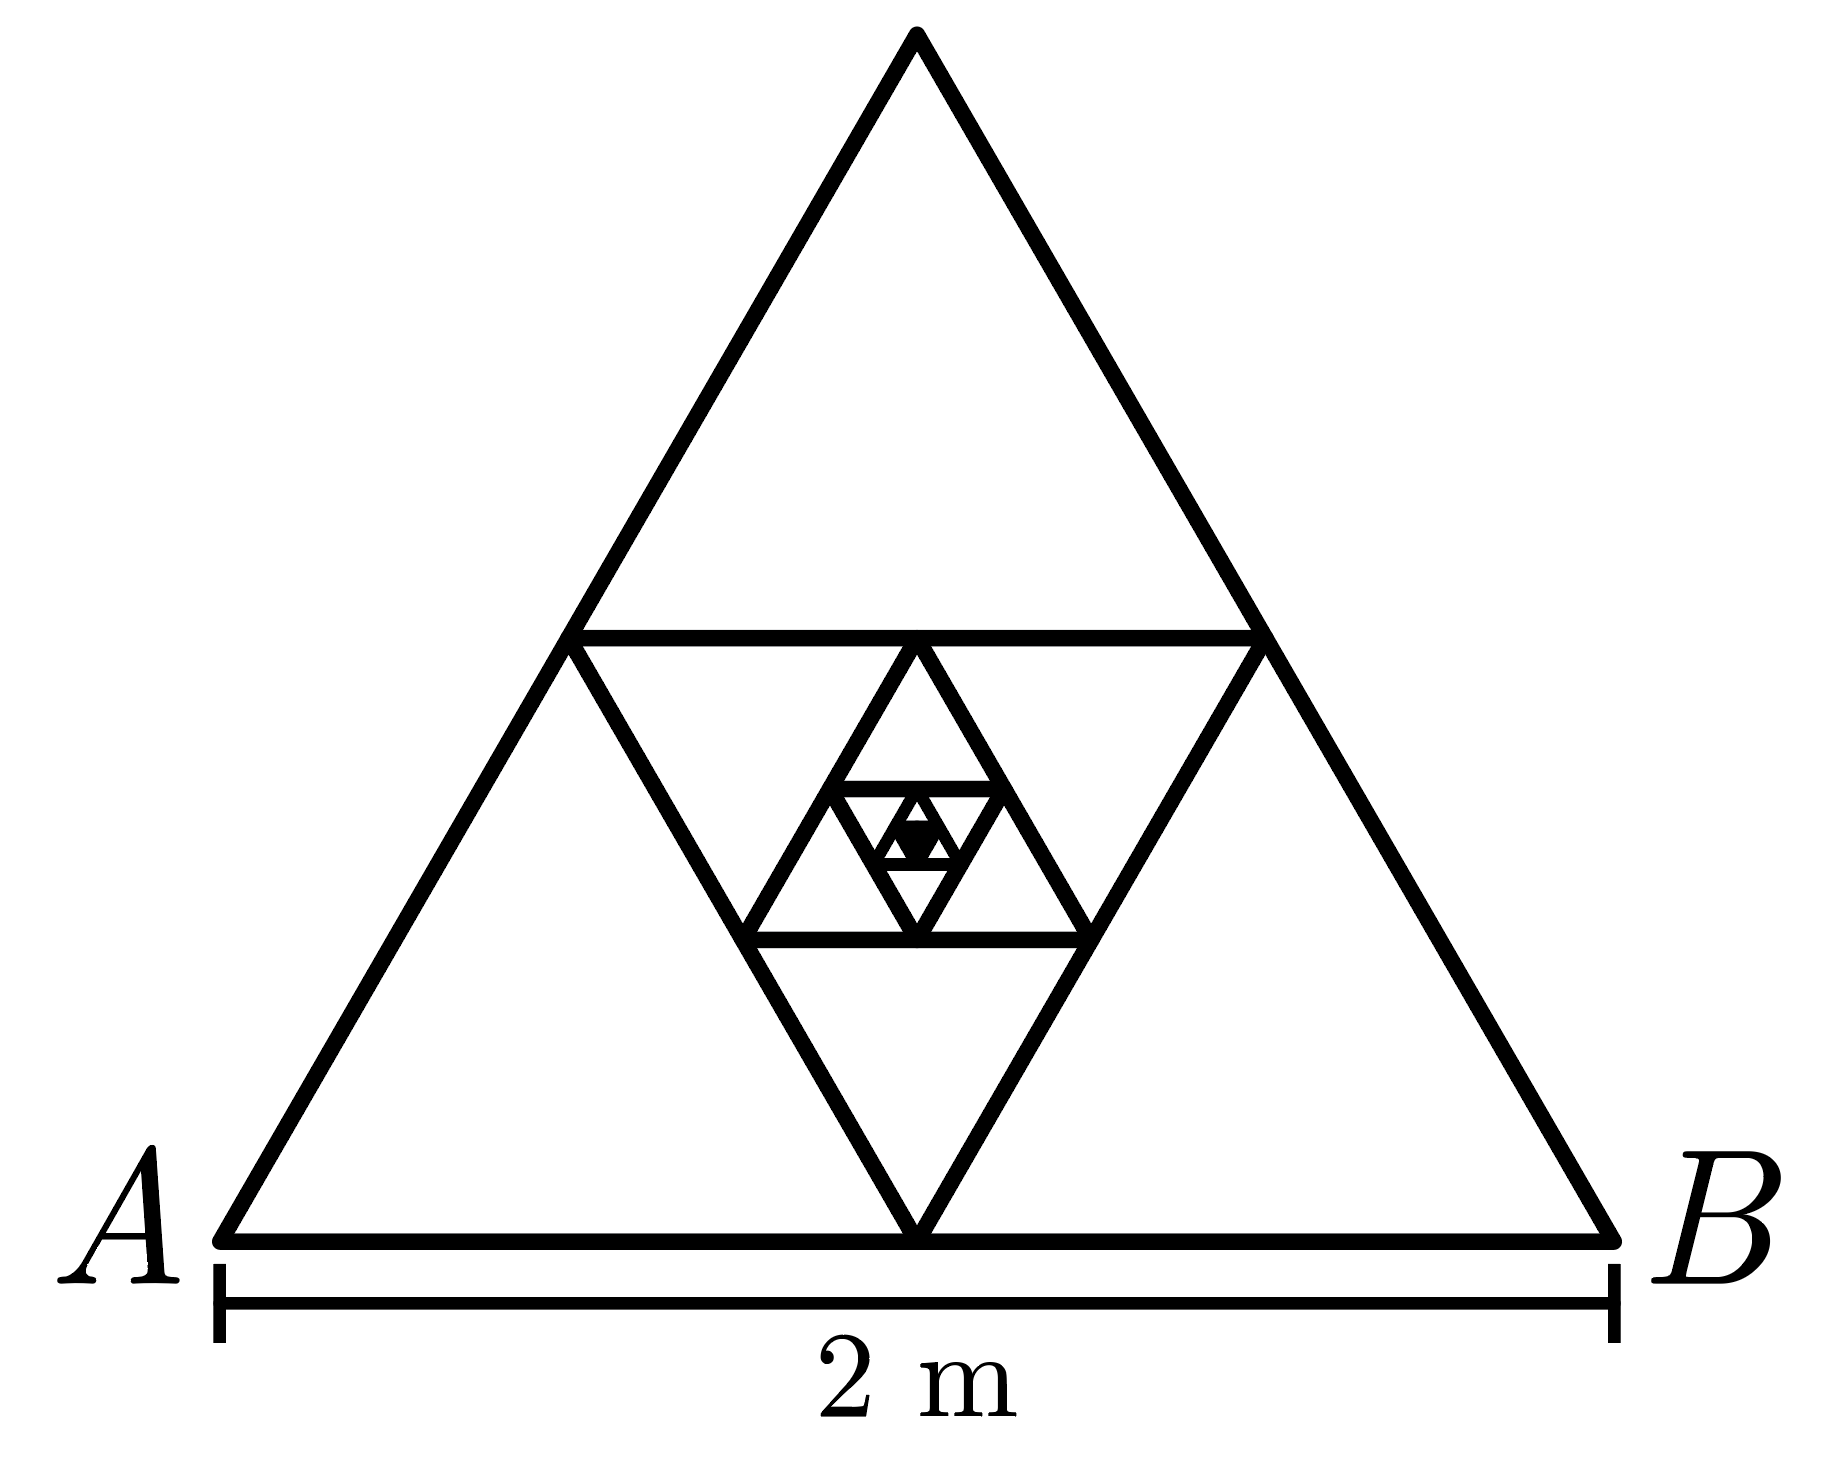
\includegraphics[width=6cm]{triangle_resistance_tesselation.png}
    \end{center}
\end{prob}
\begin{sol}
    First, using circuit trick \#1, we can disconnect the bottom connection. Then, we can use recursion to figure out the resistance. Let the resistance between $A$ and $B$ be $\eq{R}$. Then, the resistance of the smaller inner triangle, whose edges resistances are all half of that of the full triangle, must be $\eq{R}/2$. Thus, we can replace the connection between the two upper midpoints with a resistor of value $\eq{R}/2$. 

    Now, we just write down $\eq{R}$ in a second way by reducing the circuit further. This is just using series and parallel laws,
    $$\eq{R} = \frac{1}{\frac{1}{2\rho} + \frac{1}{2\rho + \frac{1}{\frac{1}{2\rho} + \frac{1}{\eq{R}/2
}}}}.$$
Ater some algebra, the above equation reduces to
$$\eq{R} = \frac{4\rho \eq R + 8 \rho^2}{3\eq R + 8\rho}.$$
Multiplying this out, we get the quadratic
$$3\eqr^2 + 4\rho \eqr - 8\rho^2 = 0,$$
which has a positive solution of
$$\eqr = \boxed{\frac{-4 +2\sqrt 7}{3}\rho}.$$
\end{sol}

\begin{prob}
    Suppose you connect two capacitors of equal capacitance $C$ in series with wires of negligible resistance, but you charge one of them up with charge $Q$ before they are connected.
    \begin{center}
        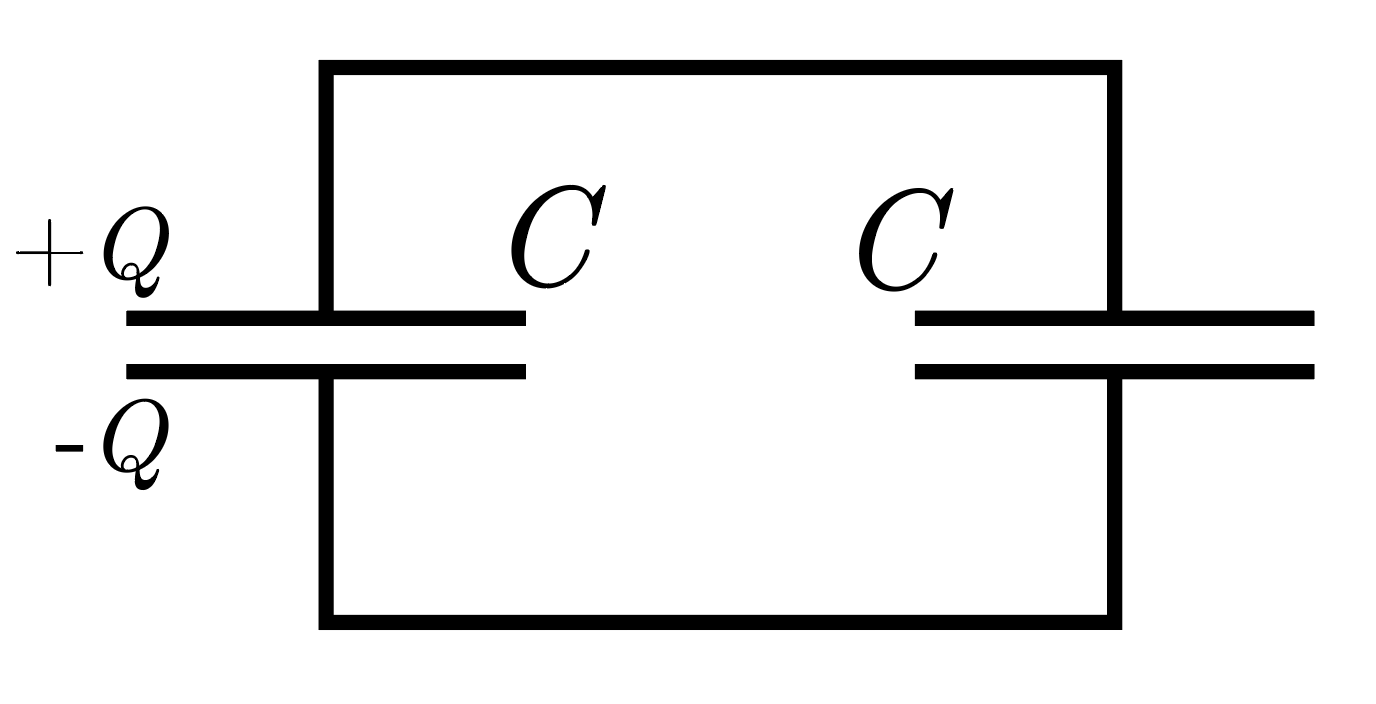
\includegraphics[width=5cm]{two_capacitor_discharge.png}
    \end{center}
    \begin{anum}
        \item After a long time, how much charge is on each capacitor?
        \item What is the change in total energy stored in the capacitors?
        \item Where does the energy loss come from? Can you show this quantitatively?
    \end{anum}
\end{prob}
\begin{alphasol}
    \item By symmetry and conservation of charge, since the voltage must be balanced on both sides, there will be $Q/2$ on each capacitor.
    \item Using the formula for energy, we have
    $$\Delta U = 2\times \frac 12 \frac{(Q/2)^2}{C} - \frac 12 \frac{Q^2}{C} = -\frac 14 \frac{Q^2}{C}.$$
    \item The trick here is that if the resistance is really small the charge will shift really quickly with high current and so the energy dissipated through the wires will still be significant. Suppose that the wires have some small resistance $r$. We can write down the following loop rule,
    $$\frac{Q_1}{C} + r \frac{dQ_1}{dt} - \frac{Q_2}{C} = 0.$$
    We have by conservation of charge $Q_1 + Q_2 = Q$, so our diffeq is
    $$\frac{2Q_1}{C} -\frac{Q}{C} + r\frac{dQ_1}{dt} = 0 \implies \frac{dQ_1}{dt} = \frac{Q-2Q_1}{rC}.$$
    Separating, we get
    $$\frac{dQ_1}{2Q_1-Q} = -\frac{dt}{rC},$$
    which gives us
    $$\frac 12 \ln\left[\frac{2Q_1 - Q}{Q}\right] = -\frac{t}{rC} \implies Q_1 = \frac{Q}{2} +\frac{Q}{2}e^{-2t/rC}.$$
    So, the current over time is
    $$I(t) = -\frac{dQ_1}{dt} = \frac{Q}{rC}e^{-2t/rC}.$$
    So, the power dissipated over time
    $$P(t) = I^2r = \frac{Q^2}{rC^2}e^{-4t/rC}.$$
    Then, integrating that we get
    $$-\Delta U = \int_0^\infty P(t) \, dt = \frac{Q^2}{rC^2}\frac{rC}{4} = \frac{Q^2}{4C},$$
    matching the energy loss in part (b).
\end{alphasol}

\begin{prob}
    Consider the interface between a wire and a resistor. There is a change in the conductivity, $\sigma_w > \sigma_r$. By conservation of charge, the current density on both sides must be the same, which means that the electric field on both sides must be different. How can this be possible? What does the circuit look like before equilibrium?
\end{prob}

\begin{sol}
    the electric field being different means that there must be a plane of charge at the interface creating the change in electric field. Where does this plane of charge come from? Initially when the electric field is continuous through the interface, the current density in the wire will be greater than that of the resistor as
    $$J_w = \sigma_w E > \sigma_r E = J_r.$$
    So, there will be more charge coming into the interface than leaving, leading to the buildup of charge which creates teh change in the electric field.
\end{sol}

\begin{prob}[Griffiths]
    Two concentric spherical conducting shells of radii $a$ and $b$ are separated by a material of resistivity $\rho$. 
    \begin{center}
        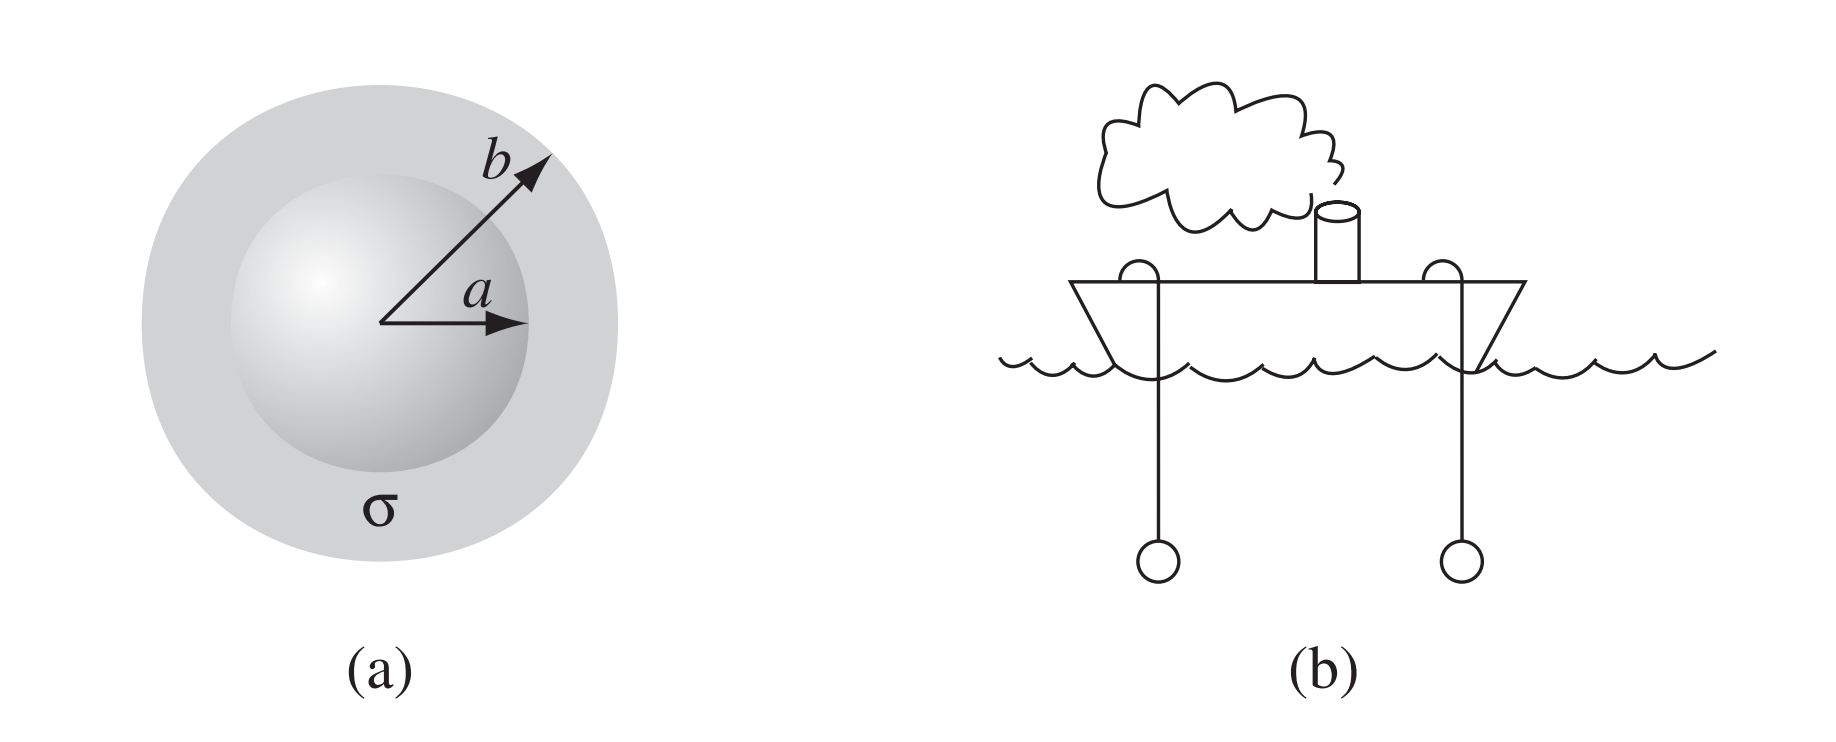
\includegraphics[width=10cm]{griffiths71.png}
    \end{center}
    \begin{anum}
        \item What is the resistance between the two shells?
        \item Now, suppose you have two metal spheres of radius $a$ separated by a distance $d \gg a$ and submerged underwater (which has resistivity $\rho$) as shown above. What is the resistance between these two spheres? \textit{Hint:} Consider the previous case with $b \gg a$. Alternatively, consider what the currents would look like with just one of the spheres at a time.
        \item (Unrelated) Now, if you removed the the material of resistivity $\rho$ in part (a) and replaced it with air, what is the capacitance between the two spherical shells?
    \end{anum}
\end{prob}

\begin{alphasol}
    \item Assume that we run a current $I$ through the inner sphere and take out $I$ from the outer sphere. Then, the current density at a radius $r$ is $J = I/(4\pi r^2)$. So, we can integrate the electric field to find the potential difference,
    $$\Delta V = -\int_a^b \frac{ I}{4\pi \sigma r^2} \, dr = \frac{I}{4\pi \sigma} \left(\frac 1a - \frac 1b \right),$$
    so the resistance is
    $$R = \frac{\Delta V}{I} = \frac{\sigma}{4\pi} \left(\frac 1a - \frac 1b\right).$$
    \item The trick here is to realize that in the case of $d \gg a$, you can consider the setup as two spherical resistors in series with $b \sim d \gg a$. This automatically gives you the answer
    $$\eqr = \frac{2}{4\pi \sigma}\left(\frac 1a - \frac 1b\right) = \boxed{\frac{\rho}{2\pi a}}.$$
    Otherwise, if you imagine $I$ going in at one sphere then the current will spread out uniformly with
    $$\mathbf J = \frac{I}{4\pi r^2} \hat r.$$
    This is precisely the shape of the field for a point charge. So, if we take out $I$ at the other sphere, the current lines will look just like that of two point charges. So, using the analogous formula, and noticing that at the surface of each sphere only the close point charge contributes to the potential significantly,
    $$\Delta V = \frac{I\rho }{4\pi a} - \frac{-I\rho}{4\pi  a} = \frac{I\rho}{2\pi a},$$
    which gives us the same result.
    \item if there is a charge $Q$ on the inner sphere, then the electric field as a function of $r$ is $E = kQ/r^2$. Thus, the potential difference is
    $$\Delta V = \int_a^b \frac{kQ}{r^2} \, dr = kQ\left(\frac 1a - \frac 1b\right).$$
    Thus, the capacitance is $C = Q/V = \frac{4\pi \epsilon_0 ab}{b-a}.$
\end{alphasol}


\begin{prob}[MPPP / USAPhO]
    Suppose that you have a conducting sphere of radius $r$ which has a charge $Q$ placed on it. It is surrounded by air which has conductivity $\sigma_{\text{air}}$.
    \begin{center}
        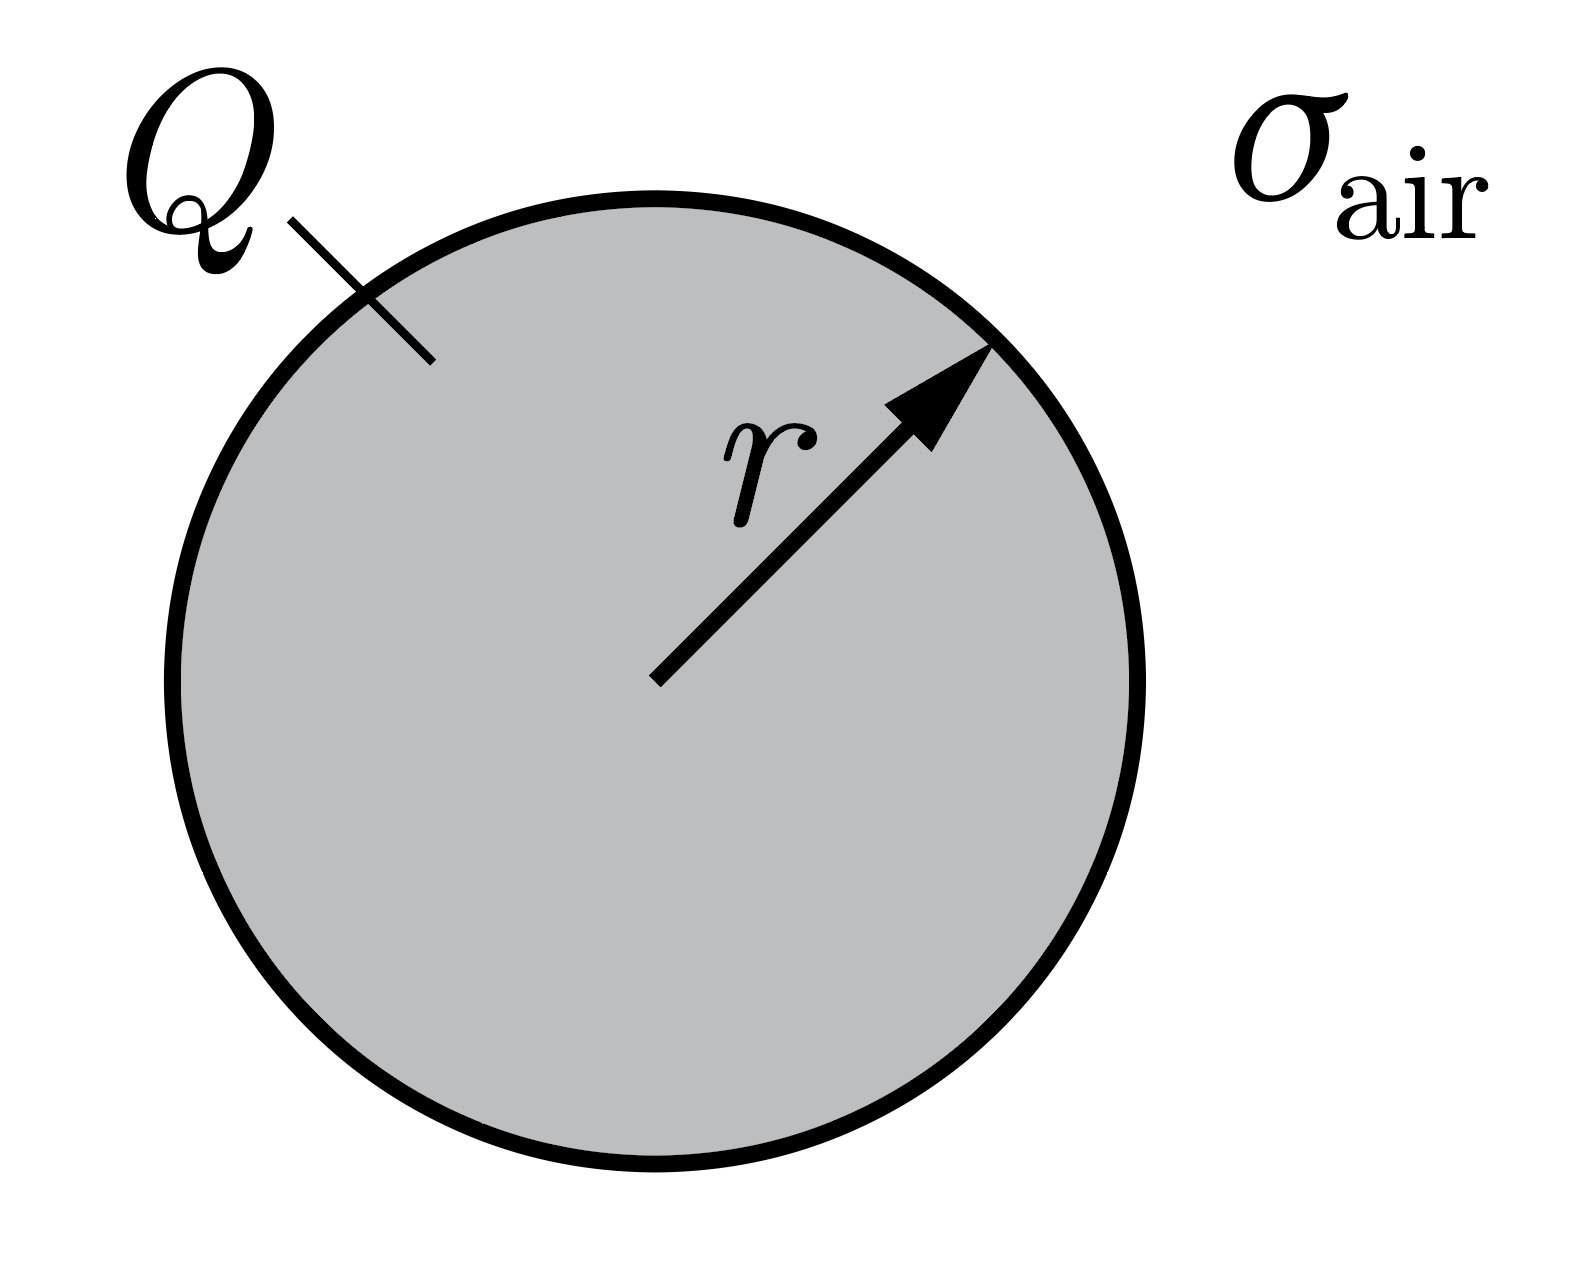
\includegraphics[width=5cm]{sphere_discharge.png}
    \end{center}
    \begin{anum}
        \item Working from first principle ($\mathbf J = \sigma \mathbf E$), find the time for the charge on the sphere to go down by a factor of $e$ due to leakage to the air.
        \item Modelling the system as an RC circuit (imagine a conducting sphere of radius $R \approx \infty \gg r$), find the time constant, and show that it matches up with part (a).
        \item Now suppose that we have an arbitrarily-shaped conductor. Show that the time for the charge on the conductor to go down by a factor of $e$ still remains the same. \textit{Hint:} Some ideas from Electrostatics may be helpful.
    \end{anum}
\end{prob}
\begin{alphasol}
    \item At the boundary of the sphere we have that
    $$\mathbf E = \frac{kQ}{r^2}\hat r \implies \mathbf J = \sigma_{\text{air}}\frac{kQ}{r^2}\hat r.$$
    Thus, the rate of change of charge on the sphere is
    $$\frac{dQ}{dt} = -J(4\pi r^2) = -\sigma_{\text{air}} (4\pi k Q).$$
    This is a first order differential equation in $Q$, which we can solve by separating, and we get
    $$Q(t) = Qe^{-4\pi k \sigma_{\text{air}}t}.$$
    Thus, reading off of the equation, the time for the charge to go down by a factor of $e$ is $\tau =\frac{1}{4\pi k \sigma_{\text{air}}} = \boxed{\frac{\epsilon_0}{\sigma_{\text{air}}}}$.
    \item Considering the hint given in the problem, we first have that the resistance is (using problem 5),
    $$R = \frac{1}{4\pi\sigma_{\text{air}}}\left(\frac 1r - \frac 1R\right) \approx \frac{1}{4\pi \sigma_{\text{air}}r}.$$
    Similarly, the capacitance is
    $$C = \frac{r}{k}.$$
    Thus, the time constant is $\tau = RC = \frac{1}{4\pi k \sigma_{\text{air}}} = \frac{\epsilon_0}{\sigma_{\text{air}}}$, matching part (a).
    \item We go back to part to the method of part (a). We have that the current density at the boundary of this surface is still
    $$\mathbf J = \sigma \mathbf E.$$
    So, the total current lost through the surface per time is given by
    $$\frac{dQ}{dt} = - \oint_S \mathbf J \cdot d\mathbf A = -\oint_S \sigma \mathbf E \cdot d\mathbf A = -\sigma \oint \mathbf E \cdot \mathbf A.$$
    But the integral is simply the flux, which we know from Gauss's law is $Q/\epsilon_0$. Thus,
    $$\frac{dQ}{dt} = -\sigma \frac{Q}{\epsilon_0},$$
    which is exactly the same differential equation as in part (a), and thus the time constant is still $\tau = \epsilon_0/\sigma_{\text{air}}$.
\end{alphasol}

\begin{prob}[Kalda]
    There is an infinite honeycomb lattice; the edges of
the lattice are made of wire, and the resistance of each edge is
$R$. Find the resistance between the two points labelled $A$ and $C$.
\begin{center}
    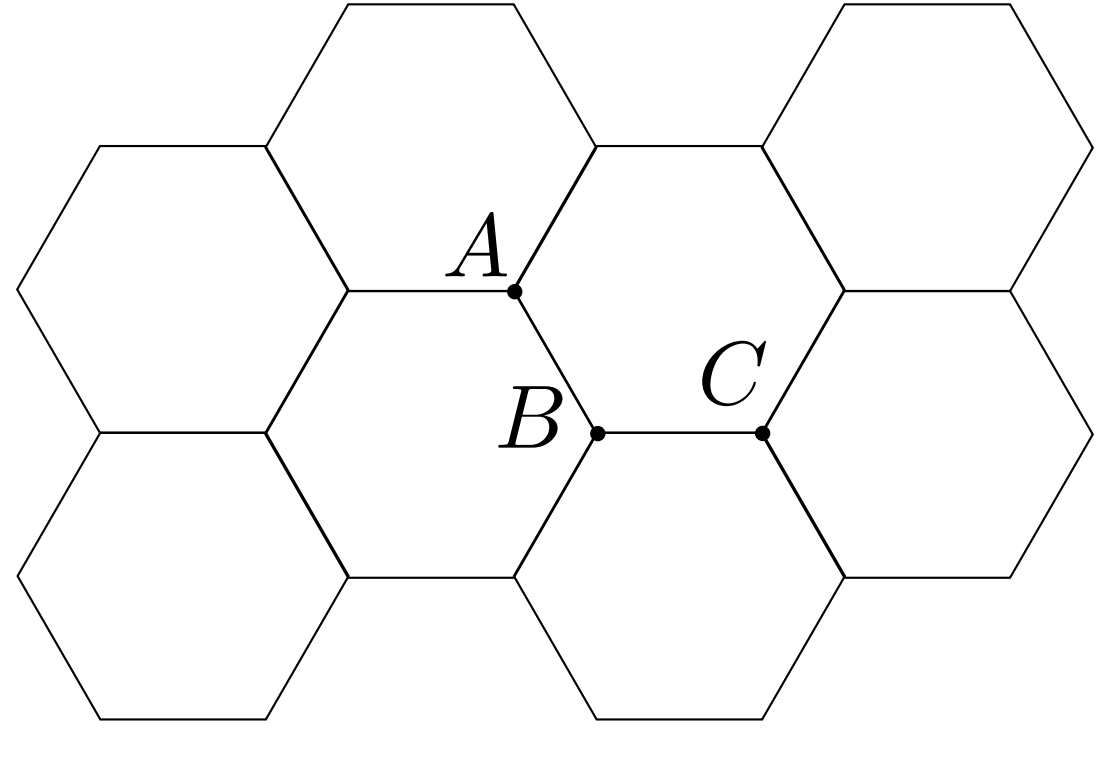
\includegraphics[width=5cm]{honeycomb_lattice.png}
\end{center}
\end{prob}

\begin{sol}
    We directly use the trick from class. Imagine injecting a current $I$ into node $A$. Then, by symmetry there wll be current $I/3$ in $\overline{AB}$ and current $I/6$ in $\overline{BC}$. Thus, the potential difference between $A$ and $C$ in this case is
    $$V_{AC}^{(\rightarrow A)} = \frac I3 R + \frac I6 R = \frac{IR}{2}.$$
    Similary, if we take out a current $I$ from $C$, we would get that
    $$V_{AC}^{(\rightarrow C)} = \frac{IR}{2}.$$
    Thus, the total potential difference in the superposition case is $V_{AC} = IR/2 +IR/2 = IR,$ and thus the equivalent resistance is $\eqr = \boxed R$.
\end{sol}

Here's another problem on finding the resistance. All the ideas used for finding the resistances of other objects work, but this might require a couple other problem solving ideas we've covered in class.

\begin{prob}[PPP]
    A plane divides space into two halves. One half is filled with homogeneous conductin medium and physicists work in the other. They mark the outline of a square of side $a$ on the plane an dlet a current $I_0$ in and out at two of its neighbouring corners using fine electrodes.
    \begin{center}
        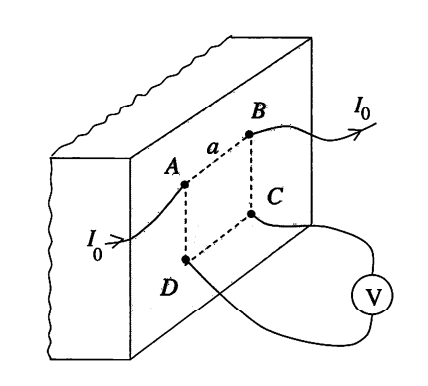
\includegraphics[width=5cm]{half_plane_resistance.png}
    \end{center}
    They measure the potential difference $V_0$ between the two other corners. What is the resistivity of the material in terms of $I_0$ and $V_0$?
\end{prob}

\begin{alphasol}
    % \item Following the strategy of the previous problem, we consider teh case where we inject $I_0$ into $A$. By symmetry it spreads out evenly over any size hemisphere in the plane. Thus, the electric field is
    % $$E(r) = \rho J(r) = \rho \frac{I_0}{2\pi r^2}.$$
    % Thus, the potential difference in this case (suppose the electrode has some small radius $\delta$)
    % $$V_{AB}^{(A)} = \frac{\rho I_0}{2\pi}\left(\frac{1}{\delta} - \frac 1r \right)$$
    \item Following the strategy of the previous problem, we consider teh case where we inject $I_0$ into $A$. By symmetry it spreads out evenly over any size hemisphere in the plane. Thus, the electric field is
    $$E(r) = \rho J(r) = \rho \frac{I_0}{2\pi r^2}.$$
    Thus, the potential difference in this case
    $$V_{DC}^{(A)} = \frac{\rho I_0}{2\pi}\left(\frac{1}{a} - \frac {\sqrt 2}{a} \right)$$
    So, the total potential difrence considering taking a curent $I_0$ out of $B$ too becomes
    $$V_0 = V_{DC} = \frac{\rho I_0}{\pi a} (1-\sqrt 2).$$
    So, the resistivity in terms of $I_0$ and $V_0$ is $\rho = \frac{V_0}{I_0} \frac{\pi a}{1 -\sqrt 2}$.
\end{alphasol}


\begin{prob}[Kalda]
    Find the thevenin equivalent EMF and resistance for the following infinite circuit below:
    \begin{center}
        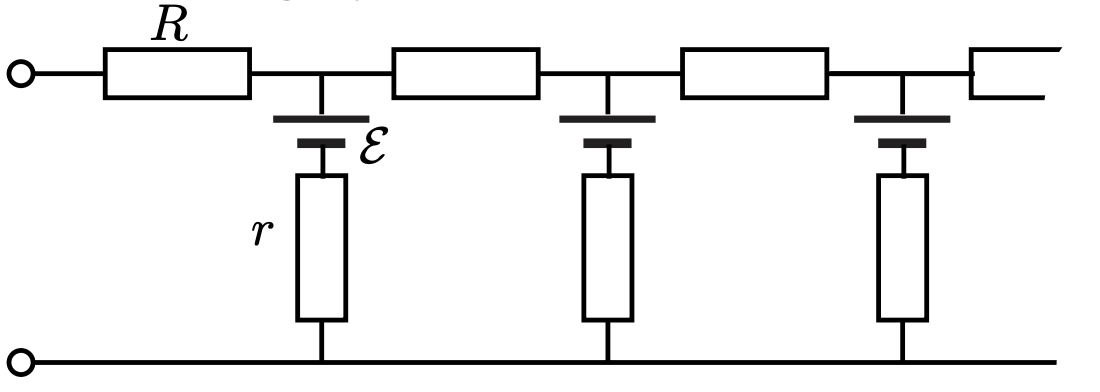
\includegraphics[width=6.5cm]{inf_thev.png}
    \end{center}
\end{prob}
\begin{sol}
    Suppose the thevenin equivalent EMF is $V$ and the equivalent resistance is $\eqr$. Then, place these two in parallel with the first section, using recursion. Now, we use the normal thevenin equivalent strategies. If we measure the voltage in the closed circuit, because the current through the right loop from Ohm's law is
    $$I = \frac{\mathcal E - V}{\eqr + r},$$
    we have that the voltage is
    $$V = \mathcal E - \frac{\mathcal E - V}{\eqr + r}r.$$
    Thus, 
    $$(V-\mathcal E) = (V - \mathcal E)\frac{r}{\eqr + r},$$
    which means that we must have $V-\mathcal E = 0 \implies \boxed{V = \mathcal E}$. Now, if we consider the short circuit case, we need to use Kirchoff's laws to figure out the current through the output nodes. Becuase the two batteries are now the same voltage, we can replace them with one and attach the wires, leaving the circuit as a battery with three resistors of equivalent resistance
    $$\eqr ' = R + \frac{1}{\frac 1r + \frac 1\eqr}.$$
    However, since we have
    $$\frac{V}{\eqr} = \frac{\mathcal E}{\eqr '} = \frac{V}{\eqr '},$$
    we have $\eqr ' = \eqr$, so
    $$\eqr = R + \frac{1}{\frac 1r + \frac 1\eqr}\implies r\eqr +\eqr ^2 = R(r + \eqr) + r\eqr.$$
    Simplifying, and using the quadratic formula, we get
    $$\boxed{\eqr = \frac{R + \sqrt{R^2 +4Rr}}{2}}.$$
\end{sol}

\begin{prob}[Kalda]
    Three identical charge-less capacitors of capacitance
$C$ are connected in series. The capacitors are charged by connecting a battery of electromotive force $\mathcal E$ to the terminal leads
of this circuit. Next, the battery is disconnected, and two resistors of resistance $R$ are connected simultaneously as shown
in figure below. Find the net heat which will be dissipated on
each of the resistances.
\begin{center}
    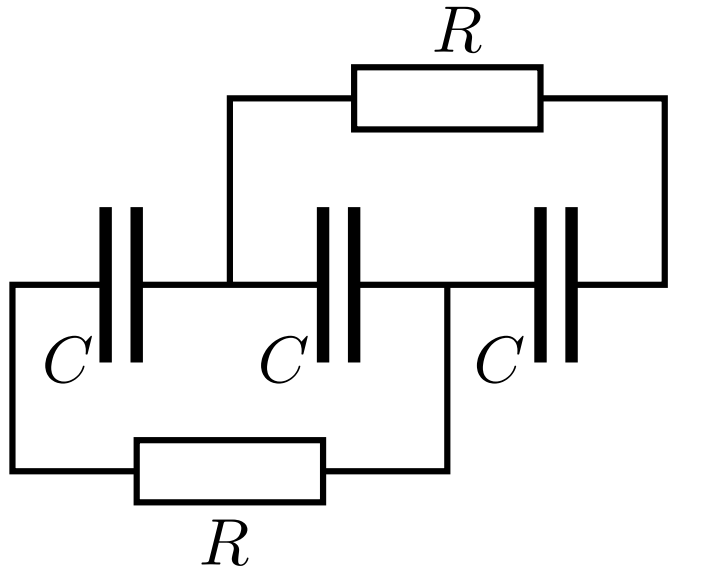
\includegraphics[width=5cm]{kalda_dissipate.png}
\end{center}
\end{prob}
\begin{sol}
    When the capacitors are charged up, since they are simply in a line, each one just has voltage $\mathcal E/3$ with charge $C\mathcal E/3$. Assume that they have positive charge on their right plates.
    
    Now, instead of actually finding the power dissipated on the resistors per time, we simply want to find what the final equilibrium state is and then find the difference in energy from the initial state. Suppose in the final state the charges on the three capacitors are $q_1,q_2,q_3$ with the value being positive if the right plate has positive charge. Then, first using the bottom loop, we get
    $$\frac{q_1}{C} + \frac{q_2}{C} = 0 \implies q_1  = -q_2.$$
    Using the top loop, we similarly get
    $$\frac{q_2}{C} + \frac{q_3}{C} = 0 \implies q_3 = -q_2 = q_1.$$
    Now, lastly, we use conservation of charge to get
    \begin{align*}
    (-q_1) + q_2 + (-q_3) &= (-C \mathcal E /3)+(C \mathcal E /3)+(-C \mathcal E /3)\\
    -3q_3 &= -C\mathcal E /3.
    \end{align*}
    So, $q_1 = q_3 = C\mathcal E / 9$ and $q_2 = -C\mathcal E/9$. So, the change in energy is
    $$\Delta U = \frac{1}{2C}\left(3\times (C\mathcal E/3)^2 - 3\times (C\mathcal E / 9)^2\right) = \frac{1}{2C}\frac{8C^2 \mathcal E^2}{27}.$$
    And each resistor dissipates half of this, so $\boxed{Q = \frac{2}{27}C\mathcal E^2}.$
\end{sol}

\begin{prob}[Purcell]
    The circuit below contains two identical capacitors and
two identical resistors. Initially, the left capacitor has charge
$Q_0$ (with the left plate positive), and the right capacitor is
uncharged. If the switch is closed at $t = 0$, find the charges
on the capacitors as functions of time. Your loop equations
should be simple ones.
\begin{center}
    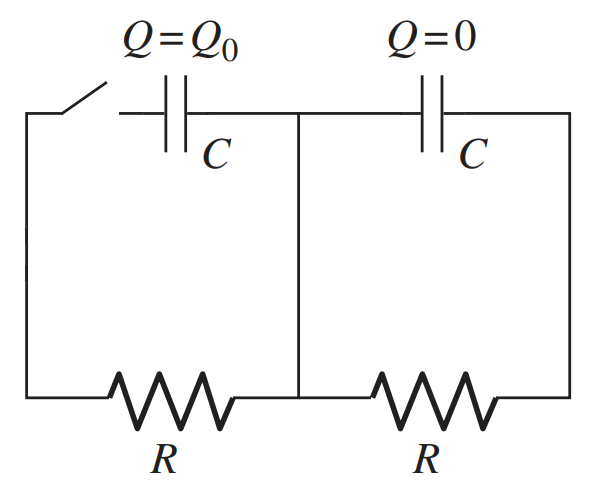
\includegraphics[width=5cm]{purcell_normal_modes.png}
\end{center}
\end{prob}

\begin{sol}
    Let $Q_1$ denote the charge on the left capacitor and $Q_2$ denote the charge on the right capacitor. The loop equation on the left is
    $$\frac{Q_1}{C} + R \frac{dQ_1}{dt} = 0,$$
    and similarly on the right loop
    $$\frac{Q_2}{C} + R\frac{dQ_2}{dt} = 0.$$
    Thus, we see that the two halves of the circuit are entirely independent, so the left side just decays on its own (this makes sense as it would skip the right half of the circuit by just flowing current through the middle wire), so we have
    \begin{align*}
        Q_1(t) &= Q_0e^{-t/RC},\\
        Q_2(t) &= 0.
    \end{align*}
\end{sol}

%could move this to usapho
% CHANGE SIGMA TO RHO IN PART D
\begin{prob}
    In this problem we explain why $\mathbf J \propto \mathbf E$ with some very rough estimations --- do not worry about any numerical factors. Model a conductor as a bunch of particles of mass $m$, charge $q$, cross-sectional area $\sigma$, and number density $n$. Suppose that each time any two of these particles collide, each particle leaves in a randomized direction with a radomized speed, which is on average $\overline{v}$.
    \begin{anum}
        \item Estimate the average distance $\lambda$ that a particle travels before colliding with a different particle. We'll touch on this more in thermodynamics.
        \item Estimate the average time betwen collisions $\tau$.
        \item Now, suppose that there is an external electric field $\mathbf E$ applied across the particles. Estimate the average \textit{velocity} over all the particles. You'll have to consider the randomized portion due to collisions along with the directional portion due to the electric field.
        \item Write down the current density and give an estimate for $\rho$ in terms of the parameters in the problem.
    \end{anum}
\end{prob}

\begin{alphasol}
    \item For simplicity, we focus on a single particle and assume that it moves through a still gel of particles with number density $n$. Then, we would like the average number of particles in the volume sweeped out by the particle as it travels a distance $\lambda$ to be order $1$. Thus, we write
    $$\sigma \lambda n \sim 1 \implies \lambda \sim \frac{1}{\sigma n}.$$
    \item Dividing the average distance by the average speed, $\tau = \frac{\lambda}{\overline v} = \frac{1}{\sigma n \overline v}.$
    \item If we focus on a single particle, around every $\tau$ it will have a randomized velocity $\mathbf u_{\text{rand}}$. And through the $\tau$ as it doesn't collide, it will be accelerated by the electric field $\mathbf E$ for an anverage time $\tau$. So, very roughly, the velocity of a single particle is
    $$\mathbf v = \mathbf u_{\text{rand}} + \frac{q\mathbf E}{m}\tau.$$
    So if we average over all particles,
    $$\langle \mathbf v \rangle = \left\langle\mathbf u_{\text{rand}} + \frac{q\mathbf E}{m}\tau\right\rangle = \langle \mathbf u_{\text{rand}}\rangle + \left\langle \frac{q\mathbf E}{m}\tau\right\rangle.$$
    The first term averages out to $0$, and the second term is a constant, so we have that the average veloctiy of the particles in this set of particles is
    $$\langle \mathbf v \rangle \sim \frac{q\mathbf E}{m}\tau.$$
    \item We can write the current density as
    $$\mathbf J = qn\mathbf v = \frac{q^2n\tau}{m}\mathbf E,$$
    giving us our desired Ohm's law form! And the proportionality constant is $\rho = \frac{m}{q^2 n \tau} = \frac{\sigma m \overline v}{q^2}.$
\end{alphasol}



\subsection{Challenge Problems}

\begin{prob}[Kalda]
    Determine the resistance between two neighbouring
vertices of a dodecahedron (see figure), the edges of which are
made of wire; the resistance of each edge is R.
\begin{center}
    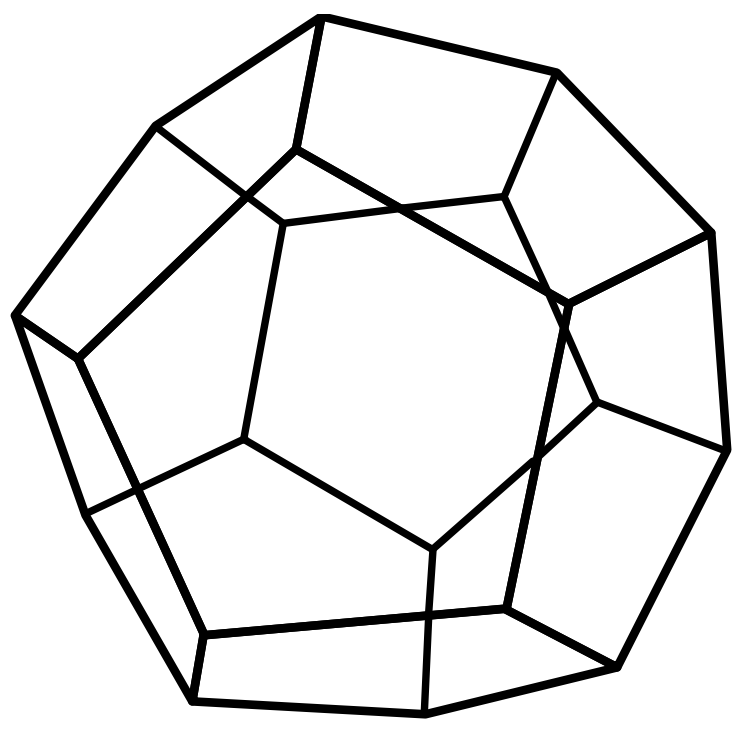
\includegraphics[width=5cm]{dodecahedron_resist.png}
\end{center}
This one's quite tricky! Make sure to ask for a hint if you need one.
\end{prob}

\begin{sol}
    We again want to use the current injection and superposition method. However, we can't simply inject current as this circuit is not infinite--there will just be charge buildup somewhere on the dodecahedron until the current can enter anymore, making it a non-static situation. So, we solve this by injecting a current $I$ into one vertex and taking out a current $I/19$ from all the other vertices. This preserves the setup. In this case, we have
    $$V_{AB}^(A) = \frac{IR}{3}, V_{AB}^(B) = \frac{IR}{3}.$$
    For vertex $B$ we take out a curent $I$ and insert a current $I/19$ into all the other vertices. Now,, if we consider the superpositions, the current gonig in and out of all vertices is $0$ except for $A$ and $B$ where it is $I + I/19 = 20I/19$. And we have
    $$V_{AB} = 2\times \frac{IR}{3},$$
    so the resistance is $R = V/I = \frac{2IR/3}{20I/19} = \frac{19R}{30}.$
\end{sol}

\begin{remark}
    Don't be scared by the ``IPhO'' label below! In fact, a lot of USAPhOs can be on par with the difficulty of IPhOs --- IPhOs are generally just longer and combine a lot of concepts. The two problems below illustrate some really cool contraptions that arise from combining a lot of physics concepts --- give them a good shot!
\end{remark}

\begin{prob}
    \href{https://ipho.olimpicos.net/pdf/IPhO_2004_Q1.pdf}{IPhO 2004, problem 1}.
\end{prob}

\begin{prob}
    \href{https://ipho.olimpicos.net/pdf/IPhO_1993_Q1.pdf}{IPhO 1993, problem 1}. 
\end{prob}


\begin{remark}
    Many of the trickiest problems in this problem set have come from the \href{https://www.ioc.ee/~kalda/ipho/electricity-circuits.pdf}{Kalda Circuits} handout. If you found them really tough, don't worry too much as the USAPhO will most likely never have a problem of this style. But they are great brain teasers!
\end{remark}

\subsection{USAPhO Practice}

Both are neuron-themed, but distinct!

\begin{prob}[USAPhO 2019/B1]
    The wall of a neuron is made from an elastic membrane, which resists compression in the same way as a spring. It has an effective spring constant $k$ and an equilibrium thickness $d_0$. Assume that the membrane has a very large area $A$ and negligible curvature. The neuron has ``ion pumps'' that can move ions across the membrane. In the resulting charged
state, positive and negative ionic charge is arranged uniformly along the outer and inner surfaces of the membrane, respectively. The permittivity of the membrane is $\epsilon$.
\begin{center}
    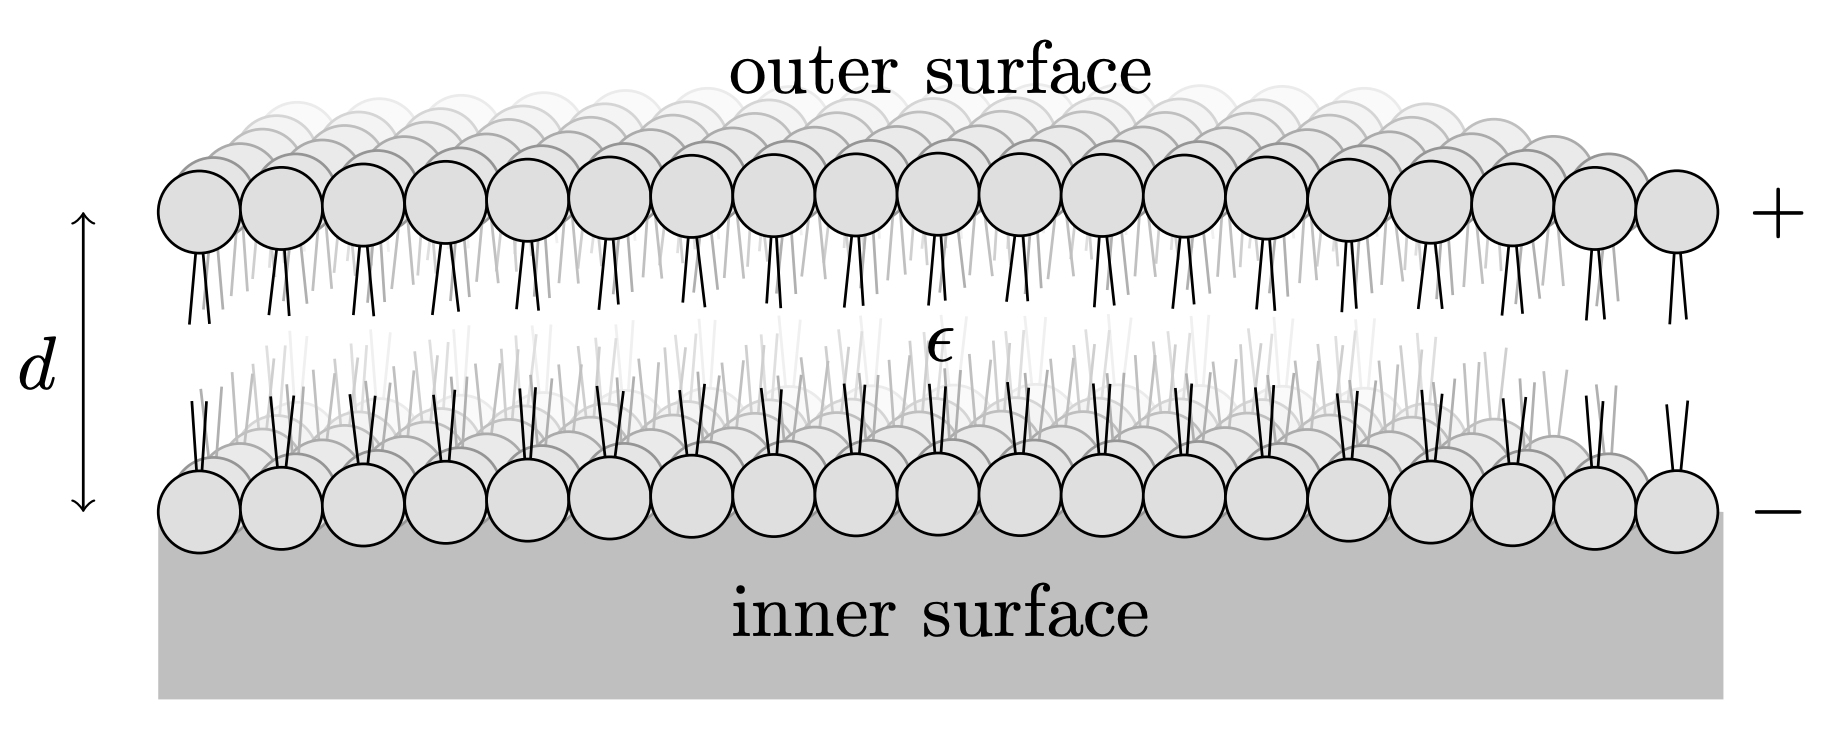
\includegraphics[width=8cm]{neuron.png}
\end{center}
\begin{anum}
    \item Suppose that, after some amount of work is done by the ion pumps, the charges on the outer
    and inner surfaces are $Q$ and $-Q$, respectively. What is the thickness $d$ of the membrane?
    \item Derive an expression for the voltage difference $V$ between the outer and inner surfaces of the
    membrane in terms of $Q$ and the other parameters given.
    \item Suppose that the ion pumps are first turned on in the uncharged state, and the membrane is
    charged very slowly (quasistatically). The pumps will only turn off when the voltage difference
    across the membrane becomes larger than a particular value $V_{\text{th}}$. How large must the spring
    constant $k$ be so that the ion pumps turn off before the membrane collapses?
    \item How much work is done by the ion pumps in each of the following situations? Express your
    answers in terms of $k$ and $d_0$.
    \begin{enumerate}[label=\roman*.]
        \item $k$ is infinitesimally larger than the value derived in part (c).
        \item $k$ is infinitesimally smaller than the value derived in part (c).
    \end{enumerate}
    Assume in each case that the membrane thickness d cannot become negative.
\end{anum}
\end{prob}

%base off of usapho+ 2021/3? do another neuron thingy that's slightly different? I want to explain the capacitor resistor combination thing and if that means its in parallel or series. -- put that either in lecture or the problem set
\begin{prob}
    When a neuron is charged up to a threshold voltage, the voltage-gated channels open and the potential difference between the inner and outer membranes. All this occurs along the axon, which we'll model as a cylinder with inner radius $a$, outer radius $b$, and length $L \gg a,b$. The space between the two cylinders is filled with a fluid of dielectric constant $\kappa$.
    \begin{center}
        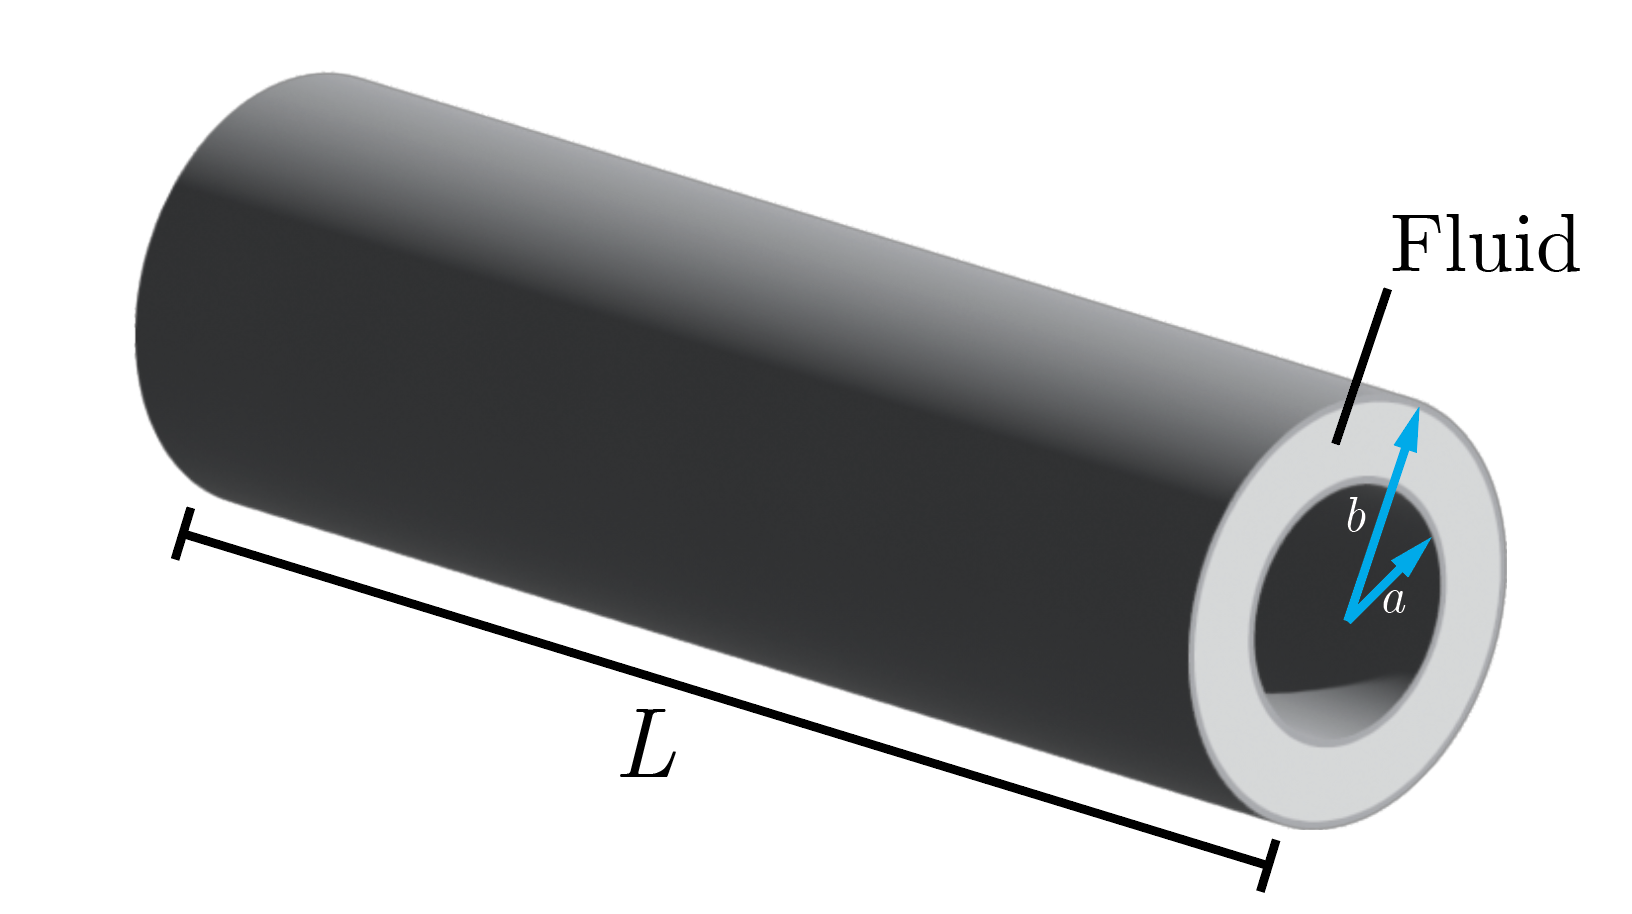
\includegraphics[width=8cm]{axon_diag.png}
    \end{center}
    

    \begin{anum}
        \item When the voltage-gated channels are opened, ions of mass $m$ and charge $q$ flow through the fluid in between. The fluid is viscous, so as they flow through, the ions experience a drag force of $F=-\eta v$. In terms of $m,q,$ or $\eta,$ what is the resistivity of the fluid?
        \item Using your result from part (a), what is the resistance $R$ between the two cylinders?
        \item What is the capacitance $C$ of the model if the inner and outer cylinders are taken as the two electrodes?
        \item Now, we model the neuron as an RC circuit.
        \begin{enumerate}[label=\roman*.]
            \item Draw the effective circuit of the neuron, comprising of the resistor and capacitor found in the previous parts and potentially additional circuit components. Explain your circuit drawing briefly and why it corresponds to the model we've developed above. In particular, be sure to explain the rationale behind any wired connections in the circuit.
            \item Estimate the time constant of the circuit.
        \end{enumerate}
    \end{anum}
\end{prob}

\begin{alphasol}
    \item Once the fluid reaches a quasi-static equilibrium, we will have that the drag froce balances out the electric force. Thus, we'll have
    $$\eta \mathbf v = q \mathbf E.$$
    Now we want to use $\mathbf v$ to figure out the current density. A set of charges with velocity $\mathbf v$ and number density $n$ passes an area $A$ with rate
    $$\frac{dN}{dt} = nAv.$$
    Thus, the current through that section is $q \frac{dN}{dt}$, which let's us write
    $$\mathbf J = \frac{I}{A} = \frac{qnA\mathbf v}{A} = qn\mathbf v = q n \frac{q\mathbf E}{\eta}.$$
    Thus, we have the proportionality constant between $\mathbf J$ and $\mathbf E$ is $q^2 n/\eta$, which is our conductivity. So, the resistivity is $\boxed{\rho = \eta / q^2n}$.
    \item If a current $I$ was injected into the inner cylinder and taken out of the outside, the current density as a function of radius in the cylinder is
    $$J(r) = \frac{I}{2\pi r L}.$$
    Thus, the change in potential difference is
    $$V = \int_a^b \frac{\rho I}{2\pi r L} = \frac{\rho I}{2\pi L}\ln(b/a),$$
    so the resistance is
    $$R = \frac{\rho}{2\pi L} \ln (b/a) = \frac{\eta }{2\pi q^2 n L}\ln (b/a).$$
    \item If we place a charge $Q$ on the inner cylinder, then, the electric field as a function of radius, incorporating the dielectric constant is,
    $$E(r) = \frac 1\kappa \frac{Q/L}{2\pi \epsilon_0 r}.$$
    Thus, the potential difference is
    $$V = \int_a^b \frac{Q}{2\pi \epsilon_0 L r}\, dr = \frac{ Q}{2\pi \kappa \epsilon_0 L}\ln(b/a).$$
    So, the capacitance is
    $$C = \frac{Q}{V} = \frac{2\pi \kappa \epsilon_0 L}{\ln (b/a)}.$$
    \item 
    \begin{enumerate}[label=\roman*.]
    \item Here's the diagram of the circuit:

    It's a bit confusing because, physically, the resistor is situated in between the two capacitor plates. However, if you actually think about the movement of charge, notice that the charge leaving the cpaacitor plates -- the outside membranes -- is equal to the amount that travels through the fluid -- the resistor. Thus, we can treat the resistor as capacitor as in a loop.
    \item This is the simplest possible $RC$ circuit, so the time constant is just
    $$\tau = RC = \frac{\eta }{2\pi q^2 n L}\ln (b/a)\frac{2\pi \kappa \epsilon_0 L}{\ln (b/a)} = \frac{\kappa \epsilon_0 \eta }{q^2 n}.$$
    \end{enumerate}
\end{alphasol}


\subsubsection{Optional, Additional Practice}

\begin{prob}
    \href{https://www.aapt.org/physicsteam/2015/upload/E3-2-5.pdf#page=4}{USAPhO 2015, A2}
\end{prob}


\end{document}